\subsection{LID and model performance}
\label{sec:performance}
In this section, we show, that LID estimates are connected with model behavior on some benchmark datasets for autoencoder and classification deep neural networks.
Our result suggests, that the connection between LID and model performance is significant, so LIDL estimates can potentially be used in problems like semi-supervised learning, active learning, uncertainty estimation, and curriculum learning.

\paragraph{Reconstruction error vs LID for autoencoders}
\begin{figure}[h]
    \centering
    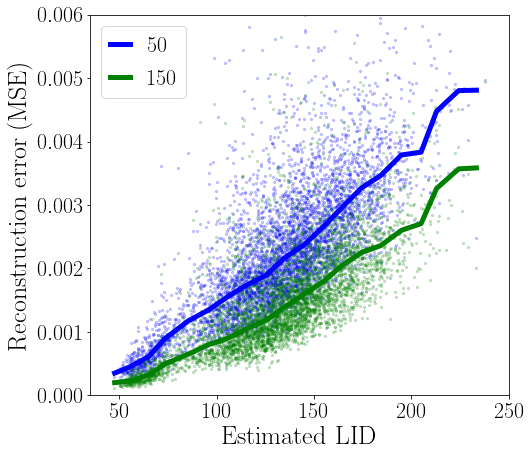
\includegraphics[width=0.45\textwidth]{images/LID-mse.png}
    \caption{LIDL estimates and VAE MSE scatterplot for a sample from MNIST dataset. Lines are running medians for those point clouds. Values in legend are VAE latent space size.}
    \label{fig:lid-mse}
\end{figure}

Results from the previous section led us to next experiment, where we wanted to investigate if the estimate from LIDL is correlated with reconstruction error for the image in VAE \citep{kingma2014auto}. We trained VAE on MNIST with latent space sizes 50 and 150, and observed that there is a high correlation (Pearsons $R > 0.7$ in both cases) between MSE and LID. We plotted LIDL estimates against MSE for 5K images in Fig.~ \ref{fig:lid-mse}. We can see an almost linear relationship between those quantities.

\paragraph{LID and classification accuracy}

We observed that classifiers can achieve better accuracy on data points with lower LID estimates. We trained neural networks on a subset of MNIST (300 images) and FMNIST (50K images) datasets and noticed a negative correlation of LID and an accuracy on a test set. Results are presented in Fig~\ref{fig:lid-accuracy}. What is more, we observed similar behavior inside a majority of classes (9 classes for MNIST, and 8 for FMNIST). 
\begin{figure}[h]
    \begin{subfigure}{.5\textwidth}
      \centering
      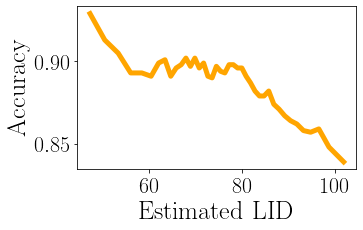
\includegraphics[width=0.6\linewidth]{images/accuracy-mnist.png}
    \end{subfigure}%
    \begin{subfigure}{.5
    \textwidth}
      \centering
      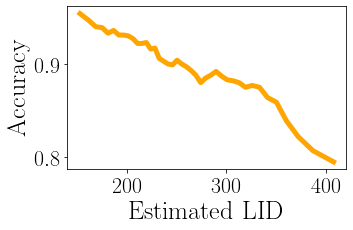
\includegraphics[width=0.6\linewidth]{images/accuracy-fmnist.png}
    \end{subfigure}
    \caption{Average classifier accuracy per LID value on MNIST(left) and FMNIST(right) datasets. We can see a very strong negative correlation between those values.}
    \label{fig:lid-accuracy}
\end{figure}

